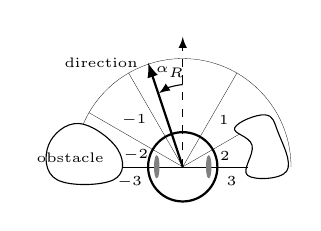
\begin{tikzpicture}[scale=0.55,font=\tiny]

% sensors
\draw [ultra thin, rotate=0](0,0) --  (1.5,0) node[near end, below]{$3$};
\draw [ultra thin, rotate=30](0,0) --  (1.5,0) node[near end, below]{$2$};;
\draw [ultra thin, rotate=60](0,0) --  (2.5,0) node[midway, right]{$1$};;
\draw [ultra thin, rotate=120](0,0) --  (2.5,0) node[midway, left]{$-1$};;
\draw [ultra thin, rotate=150](0,0) --  (2.5,0) node[midway, below]{$-2$};;
\draw [ultra thin, rotate=180](0,0) --  (1.4,0) node[very near end, below]{$-3$};;
% direction 
\draw [thick,-latex](0,0) --  (-0.8,2.4) node[at end, left]{direction};
% angle
\draw [-latex](0,1.9) arc (95.9158:124.2285:1.2) node[midway,above]{$\alpha_R$};
\draw [dashed,-latex](0,0) --  (0,3) node[at end, right]{};
% robot
\draw [thick] (0,0) ellipse (0.8 and 0.8);
% wheels
\draw  [fill,gray, rotate around={90:(0.6,0)} ]  (0.6,0) node (v1) {} ellipse (0.25 and 0.05);
\draw  [fill,gray, rotate around={90:(-0.6,0)} ]  (-0.6,0) node (v2) {} ellipse (0.25 and 0.05);
% obstacles
\draw  plot[smooth cycle, tension=.7] coordinates {(-1.5,0.4) (-2.4,1) (-3.1,0.5) (-2.9,-0.3) (-1.6,-0.3)} node[below=-8,left]{obstacle};
\draw  plot[smooth cycle, tension=.7] coordinates {(1.2,0.9) (1.6,0.5) (1.5,-0.2) (2.4,-0.1) (2.2,0.8) (1.9,1.2)};
%circle
\draw [ultra thin] (2.5,0) arc (0:157:2.5);

\end{tikzpicture}